% Options for packages loaded elsewhere
\PassOptionsToPackage{unicode}{hyperref}
\PassOptionsToPackage{hyphens}{url}
%
\documentclass[
]{article}
\usepackage{amsmath,amssymb}
\usepackage{lmodern}
\usepackage{iftex}
\ifPDFTeX
  \usepackage[T1]{fontenc}
  \usepackage[utf8]{inputenc}
  \usepackage{textcomp} % provide euro and other symbols
\else % if luatex or xetex
  \usepackage{unicode-math}
  \defaultfontfeatures{Scale=MatchLowercase}
  \defaultfontfeatures[\rmfamily]{Ligatures=TeX,Scale=1}
\fi
% Use upquote if available, for straight quotes in verbatim environments
\IfFileExists{upquote.sty}{\usepackage{upquote}}{}
\IfFileExists{microtype.sty}{% use microtype if available
  \usepackage[]{microtype}
  \UseMicrotypeSet[protrusion]{basicmath} % disable protrusion for tt fonts
}{}
\makeatletter
\@ifundefined{KOMAClassName}{% if non-KOMA class
  \IfFileExists{parskip.sty}{%
    \usepackage{parskip}
  }{% else
    \setlength{\parindent}{0pt}
    \setlength{\parskip}{6pt plus 2pt minus 1pt}}
}{% if KOMA class
  \KOMAoptions{parskip=half}}
\makeatother
\usepackage{xcolor}
\IfFileExists{xurl.sty}{\usepackage{xurl}}{} % add URL line breaks if available
\IfFileExists{bookmark.sty}{\usepackage{bookmark}}{\usepackage{hyperref}}
\hypersetup{
  pdftitle={Statistik und Qualität - Ausarbeitung der vierten Übung},
  pdfauthor={Stefan Dünser},
  hidelinks,
  pdfcreator={LaTeX via pandoc}}
\urlstyle{same} % disable monospaced font for URLs
\usepackage[margin=1in]{geometry}
\usepackage{color}
\usepackage{fancyvrb}
\newcommand{\VerbBar}{|}
\newcommand{\VERB}{\Verb[commandchars=\\\{\}]}
\DefineVerbatimEnvironment{Highlighting}{Verbatim}{commandchars=\\\{\}}
% Add ',fontsize=\small' for more characters per line
\usepackage{framed}
\definecolor{shadecolor}{RGB}{248,248,248}
\newenvironment{Shaded}{\begin{snugshade}}{\end{snugshade}}
\newcommand{\AlertTok}[1]{\textcolor[rgb]{0.94,0.16,0.16}{#1}}
\newcommand{\AnnotationTok}[1]{\textcolor[rgb]{0.56,0.35,0.01}{\textbf{\textit{#1}}}}
\newcommand{\AttributeTok}[1]{\textcolor[rgb]{0.77,0.63,0.00}{#1}}
\newcommand{\BaseNTok}[1]{\textcolor[rgb]{0.00,0.00,0.81}{#1}}
\newcommand{\BuiltInTok}[1]{#1}
\newcommand{\CharTok}[1]{\textcolor[rgb]{0.31,0.60,0.02}{#1}}
\newcommand{\CommentTok}[1]{\textcolor[rgb]{0.56,0.35,0.01}{\textit{#1}}}
\newcommand{\CommentVarTok}[1]{\textcolor[rgb]{0.56,0.35,0.01}{\textbf{\textit{#1}}}}
\newcommand{\ConstantTok}[1]{\textcolor[rgb]{0.00,0.00,0.00}{#1}}
\newcommand{\ControlFlowTok}[1]{\textcolor[rgb]{0.13,0.29,0.53}{\textbf{#1}}}
\newcommand{\DataTypeTok}[1]{\textcolor[rgb]{0.13,0.29,0.53}{#1}}
\newcommand{\DecValTok}[1]{\textcolor[rgb]{0.00,0.00,0.81}{#1}}
\newcommand{\DocumentationTok}[1]{\textcolor[rgb]{0.56,0.35,0.01}{\textbf{\textit{#1}}}}
\newcommand{\ErrorTok}[1]{\textcolor[rgb]{0.64,0.00,0.00}{\textbf{#1}}}
\newcommand{\ExtensionTok}[1]{#1}
\newcommand{\FloatTok}[1]{\textcolor[rgb]{0.00,0.00,0.81}{#1}}
\newcommand{\FunctionTok}[1]{\textcolor[rgb]{0.00,0.00,0.00}{#1}}
\newcommand{\ImportTok}[1]{#1}
\newcommand{\InformationTok}[1]{\textcolor[rgb]{0.56,0.35,0.01}{\textbf{\textit{#1}}}}
\newcommand{\KeywordTok}[1]{\textcolor[rgb]{0.13,0.29,0.53}{\textbf{#1}}}
\newcommand{\NormalTok}[1]{#1}
\newcommand{\OperatorTok}[1]{\textcolor[rgb]{0.81,0.36,0.00}{\textbf{#1}}}
\newcommand{\OtherTok}[1]{\textcolor[rgb]{0.56,0.35,0.01}{#1}}
\newcommand{\PreprocessorTok}[1]{\textcolor[rgb]{0.56,0.35,0.01}{\textit{#1}}}
\newcommand{\RegionMarkerTok}[1]{#1}
\newcommand{\SpecialCharTok}[1]{\textcolor[rgb]{0.00,0.00,0.00}{#1}}
\newcommand{\SpecialStringTok}[1]{\textcolor[rgb]{0.31,0.60,0.02}{#1}}
\newcommand{\StringTok}[1]{\textcolor[rgb]{0.31,0.60,0.02}{#1}}
\newcommand{\VariableTok}[1]{\textcolor[rgb]{0.00,0.00,0.00}{#1}}
\newcommand{\VerbatimStringTok}[1]{\textcolor[rgb]{0.31,0.60,0.02}{#1}}
\newcommand{\WarningTok}[1]{\textcolor[rgb]{0.56,0.35,0.01}{\textbf{\textit{#1}}}}
\usepackage{graphicx}
\makeatletter
\def\maxwidth{\ifdim\Gin@nat@width>\linewidth\linewidth\else\Gin@nat@width\fi}
\def\maxheight{\ifdim\Gin@nat@height>\textheight\textheight\else\Gin@nat@height\fi}
\makeatother
% Scale images if necessary, so that they will not overflow the page
% margins by default, and it is still possible to overwrite the defaults
% using explicit options in \includegraphics[width, height, ...]{}
\setkeys{Gin}{width=\maxwidth,height=\maxheight,keepaspectratio}
% Set default figure placement to htbp
\makeatletter
\def\fps@figure{htbp}
\makeatother
\setlength{\emergencystretch}{3em} % prevent overfull lines
\providecommand{\tightlist}{%
  \setlength{\itemsep}{0pt}\setlength{\parskip}{0pt}}
\setcounter{secnumdepth}{-\maxdimen} % remove section numbering
\ifLuaTeX
  \usepackage{selnolig}  % disable illegal ligatures
\fi

\title{Statistik und Qualität - Ausarbeitung der vierten Übung}
\author{Stefan Dünser}
\date{}

\begin{document}
\maketitle

\#\#\# B-1) Ein Produktionsbetrieb arbeitet mit Maschinen, die einen
Verschleißteil T enthalten. Die typischen, für den Teil T beobachteten
Lebensdauern waren in 4000 Fällen:

\begin{Shaded}
\begin{Highlighting}[]
\CommentTok{\# Erstellen einer Liste mit den Werten aus der Angabe}
\NormalTok{Verschleissteile.df }\OtherTok{\textless{}{-}} \FunctionTok{data.frame}\NormalTok{(}\AttributeTok{KlassenLebensdauer =} \FunctionTok{c}\NormalTok{(}\StringTok{"[2750,3250]"}\NormalTok{,}\StringTok{"]3250,3750]"}\NormalTok{,}\StringTok{"]3750,4250]"}\NormalTok{,}\StringTok{"]4250,4750]"}\NormalTok{,}\StringTok{"]4750,5250]"}\NormalTok{,}\StringTok{"]5250,5750]"}\NormalTok{,}\StringTok{"]5750,6250]"}\NormalTok{,}\StringTok{"]6250,6750]"}\NormalTok{, }\StringTok{"]6750,7250]"}\NormalTok{), }\AttributeTok{Klassenbreite =} \FunctionTok{rep}\NormalTok{(}\FloatTok{500.00}\NormalTok{,}\DecValTok{9}\NormalTok{), }\AttributeTok{Klassenmitte =} \FunctionTok{c}\NormalTok{(}\FloatTok{3000.00}\NormalTok{,}\FloatTok{3500.00}\NormalTok{,}\FloatTok{4000.00}\NormalTok{,}\FloatTok{4500.00}\NormalTok{,}\FloatTok{5000.00}\NormalTok{,}\FloatTok{5500.00}\NormalTok{,}\FloatTok{6000.00}\NormalTok{,}\FloatTok{6500.00}\NormalTok{,}\FloatTok{7000.00}\NormalTok{), }\AttributeTok{Anzahl =} \FunctionTok{c}\NormalTok{(}\DecValTok{160}\NormalTok{,}\DecValTok{240}\NormalTok{,}\DecValTok{400}\NormalTok{,}\DecValTok{600}\NormalTok{,}\DecValTok{1200}\NormalTok{,}\DecValTok{800}\NormalTok{,}\DecValTok{320}\NormalTok{,}\DecValTok{200}\NormalTok{,}\DecValTok{80}\NormalTok{))}
\NormalTok{  Verschleissteile.df}
\end{Highlighting}
\end{Shaded}

\begin{verbatim}
##   KlassenLebensdauer Klassenbreite Klassenmitte Anzahl
## 1        [2750,3250]           500         3000    160
## 2        ]3250,3750]           500         3500    240
## 3        ]3750,4250]           500         4000    400
## 4        ]4250,4750]           500         4500    600
## 5        ]4750,5250]           500         5000   1200
## 6        ]5250,5750]           500         5500    800
## 7        ]5750,6250]           500         6000    320
## 8        ]6250,6750]           500         6500    200
## 9        ]6750,7250]           500         7000     80
\end{verbatim}

\textbf{Schätze die Wahrscheinlichkeiten für die Lebensdauer des Teiles
T in den gegebenen Klassenbreiten.} Aus der tabellarischen Darstellung
geht hervor, dass die meisten Teile in der Mitte der Verteilung zu
finden ist (KlasseLebensdauer ``{]}4750,5250{]}''). Dies deutet darauf
hin, dass der Schwerpunkt der Verteilung bei der erwähnten
KlassenLebensdauer liegt. Der Schwerpunkt wiederum symbolisiert wiederum
das arithmetische Mittel der Vereteilung. Geschätzt liegt das
arithmetische Mittel bei rund 5000 h.

\begin{Shaded}
\begin{Highlighting}[]
\FunctionTok{par}\NormalTok{(}\AttributeTok{las =} \DecValTok{2}\NormalTok{)    }\CommentTok{\# Anordnen der Beschriftung der Klassenbreiten (Intervalle) vertikal}
\FunctionTok{barplot}\NormalTok{(Verschleissteile.df}\SpecialCharTok{$}\NormalTok{Anzahl, }\AttributeTok{names.arg =}\NormalTok{ Verschleissteile.df}\SpecialCharTok{$}\NormalTok{KlassenLebensdauer, }\AttributeTok{ylab =} \StringTok{"Anzahl der Teile"}\NormalTok{, }\AttributeTok{main =} \StringTok{"Lebensdauer eines Teils"}\NormalTok{, }\AttributeTok{col =} \StringTok{"blue"}\NormalTok{)}
\end{Highlighting}
\end{Shaded}

\includegraphics{Uebung4_StefanDuenser_files/figure-latex/unnamed-chunk-2-1.pdf}
Auch anhand der grafischen Darstellung kann der Schwerpunkt und somit
das arithmetische Mittel der Verteilung auf ca. 5000 h geschätzt werden.
~\\
\textbf{Berechne die mittlere Lebensdauer (Erwartungswert) und die
Streuung (Standardabweichung) der Lebensdauer (in Stunden). (µ = 4950
Std, s = 867 Std)}\\
\textbf{Erwartungswert:}\\

\begin{Shaded}
\begin{Highlighting}[]
\NormalTok{Erwartungswert }\OtherTok{\textless{}{-}} \FunctionTok{sum}\NormalTok{(Verschleissteile.df}\SpecialCharTok{$}\NormalTok{Klassenmitte}\SpecialCharTok{*}\NormalTok{(Verschleissteile.df}\SpecialCharTok{$}\NormalTok{Anzahl}\SpecialCharTok{/}\FunctionTok{sum}\NormalTok{(Verschleissteile.df}\SpecialCharTok{$}\NormalTok{Anzahl)))}
\NormalTok{Erwartungswert}
\end{Highlighting}
\end{Shaded}

\begin{verbatim}
## [1] 4950
\end{verbatim}

\textbf{Standardabweichung:}\\

\begin{Shaded}
\begin{Highlighting}[]
\NormalTok{n.vec }\OtherTok{\textless{}{-}}\NormalTok{ Verschleissteile.df}\SpecialCharTok{$}\NormalTok{Anzahl}\SpecialCharTok{/}\FunctionTok{sum}\NormalTok{(Verschleissteile.df}\SpecialCharTok{$}\NormalTok{Anzahl)}
\NormalTok{Standardabweichung }\OtherTok{\textless{}{-}} \FunctionTok{sqrt}\NormalTok{(}\FunctionTok{sum}\NormalTok{((Verschleissteile.df}\SpecialCharTok{$}\NormalTok{Klassenmitte}\SpecialCharTok{{-}}\NormalTok{Erwartungswert)}\SpecialCharTok{\^{}}\DecValTok{2}\SpecialCharTok{*}\NormalTok{n.vec))}
\NormalTok{Standardabweichung}
\end{Highlighting}
\end{Shaded}

\begin{verbatim}
## [1] 867.4676
\end{verbatim}

\textbf{Stelle die Wahrscheinlichkeitsfunktion und die
Verteilungsfunktion (Summenhäufigkeit) graphisch dar.}\\

\begin{Shaded}
\begin{Highlighting}[]
\CommentTok{\# Berechnen der Summenhäufigkeit und der relativen Häufigkeit}
\NormalTok{SummenHfk.vec }\OtherTok{\textless{}{-}} \FunctionTok{cumsum}\NormalTok{(Verschleissteile.df}\SpecialCharTok{$}\NormalTok{Anzahl)}\SpecialCharTok{/}\FunctionTok{sum}\NormalTok{(Verschleissteile.df}\SpecialCharTok{$}\NormalTok{Anzahl)}
\NormalTok{Haeufigkeit.vec }\OtherTok{\textless{}{-}}\NormalTok{ Verschleissteile.df}\SpecialCharTok{$}\NormalTok{Anzahl}\SpecialCharTok{/}\FunctionTok{sum}\NormalTok{(Verschleissteile.df}\SpecialCharTok{$}\NormalTok{Anzahl)}
\CommentTok{\# Ergänzen der Werteliste aus der Angabe um die berechneten Werte}
\NormalTok{Verschleissteile.df }\OtherTok{\textless{}{-}} \FunctionTok{data.frame}\NormalTok{(Verschleissteile.df, }\AttributeTok{SummenHfk =}\NormalTok{ SummenHfk.vec, }\AttributeTok{Haeufigkeit =}\NormalTok{ Haeufigkeit.vec)}
\NormalTok{Verschleissteile.df}
\end{Highlighting}
\end{Shaded}

\begin{verbatim}
##   KlassenLebensdauer Klassenbreite Klassenmitte Anzahl SummenHfk Haeufigkeit
## 1        [2750,3250]           500         3000    160      0.04        0.04
## 2        ]3250,3750]           500         3500    240      0.10        0.06
## 3        ]3750,4250]           500         4000    400      0.20        0.10
## 4        ]4250,4750]           500         4500    600      0.35        0.15
## 5        ]4750,5250]           500         5000   1200      0.65        0.30
## 6        ]5250,5750]           500         5500    800      0.85        0.20
## 7        ]5750,6250]           500         6000    320      0.93        0.08
## 8        ]6250,6750]           500         6500    200      0.98        0.05
## 9        ]6750,7250]           500         7000     80      1.00        0.02
\end{verbatim}

\textbf{Wahrscheinlichkeitsfunktion:}\\

\begin{Shaded}
\begin{Highlighting}[]
\FunctionTok{par}\NormalTok{(}\AttributeTok{las =} \DecValTok{2}\NormalTok{)    }\CommentTok{\# Anordnen der Beschriftung der Klassenbreiten (Intervalle) vertikal}
\FunctionTok{barplot}\NormalTok{(Verschleissteile.df}\SpecialCharTok{$}\NormalTok{Haeufigkeit, }\AttributeTok{names.arg =}\NormalTok{ Verschleissteile.df}\SpecialCharTok{$}\NormalTok{KlassenLebensdauer, }\AttributeTok{ylab =} \StringTok{"rel. Häufigkeit"}\NormalTok{, }\AttributeTok{main =} \StringTok{"Lebensdauer eines Teils"}\NormalTok{, }\AttributeTok{col =} \StringTok{"blue"}\NormalTok{, }\AttributeTok{ylim =} \FunctionTok{c}\NormalTok{(}\FloatTok{0.00}\NormalTok{,}\FloatTok{0.35}\NormalTok{))}
\end{Highlighting}
\end{Shaded}

\includegraphics{Uebung4_StefanDuenser_files/figure-latex/unnamed-chunk-6-1.pdf}

\textbf{Verteilungsfunktion (Summenhäufigkeit):}\\

\begin{Shaded}
\begin{Highlighting}[]
\NormalTok{Breaks.vec }\OtherTok{\textless{}{-}} \FunctionTok{c}\NormalTok{(}\DecValTok{3000}\NormalTok{,}\DecValTok{3500}\NormalTok{,}\DecValTok{4000}\NormalTok{,}\DecValTok{4500}\NormalTok{,}\DecValTok{5000}\NormalTok{,}\DecValTok{5500}\NormalTok{,}\DecValTok{6000}\NormalTok{,}\DecValTok{6500}\NormalTok{,}\DecValTok{7000}\NormalTok{)}
\FunctionTok{plot}\NormalTok{(Breaks.vec, Verschleissteile.df}\SpecialCharTok{$}\NormalTok{SummenHfk,}\AttributeTok{type =} \StringTok{"l"}\NormalTok{, }\AttributeTok{lty =} \DecValTok{1}\NormalTok{, , }\AttributeTok{main =} \StringTok{"Summenhäufigkeit der Verschleißteilelebensdauer"}\NormalTok{, }\AttributeTok{xlab =} \StringTok{"Lebensdauer in h"}\NormalTok{, }\AttributeTok{ylab =} \StringTok{"relative Häufigkeit"}\NormalTok{)}
\FunctionTok{points}\NormalTok{(Breaks.vec, Verschleissteile.df}\SpecialCharTok{$}\NormalTok{SummenHfk) }\CommentTok{\# Darstellung der Messpunkte als Punkte}
\FunctionTok{lines}\NormalTok{(Breaks.vec, Verschleissteile.df}\SpecialCharTok{$}\NormalTok{SummenHfk, }\AttributeTok{type =} \StringTok{"s"}\NormalTok{, }\AttributeTok{lty =} \DecValTok{3}\NormalTok{) }\CommentTok{\# Darstellung der Steigungsdreiecke}
\FunctionTok{abline}\NormalTok{(}\FloatTok{0.25}\NormalTok{, }\DecValTok{0}\NormalTok{, }\AttributeTok{lty =} \StringTok{"dashed"}\NormalTok{)               }\CommentTok{\# unteres Quartil}
\FunctionTok{abline}\NormalTok{(}\FloatTok{0.5}\NormalTok{, }\DecValTok{0}\NormalTok{, }\AttributeTok{lty =} \StringTok{"dashed"}\NormalTok{, }\AttributeTok{col =} \StringTok{"red"}\NormalTok{)   }\CommentTok{\# Median}
\FunctionTok{abline}\NormalTok{(}\FloatTok{0.75}\NormalTok{, }\DecValTok{0}\NormalTok{, }\AttributeTok{lty =} \StringTok{"dashed"}\NormalTok{)               }\CommentTok{\# oberes Quartil}
\end{Highlighting}
\end{Shaded}

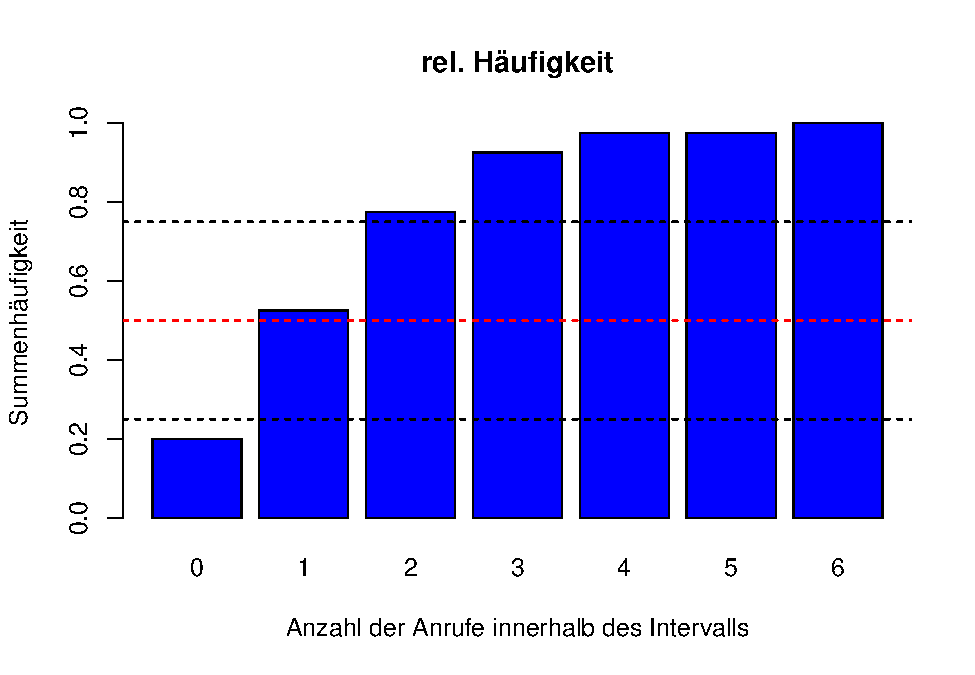
\includegraphics{Uebung4_StefanDuenser_files/figure-latex/unnamed-chunk-7-1.pdf}
\#\#\# B-2) Erzeuge 500 Zufallszahlen, welche die Lebensdauern von 500
Teilen T simulieren (und somit der Verteilung aus Aufgabe B-1
entsprechen).

\begin{Shaded}
\begin{Highlighting}[]
\CommentTok{\# Mit der Variable "AnzahlZufallszahlen" gibt man der Funktion mit, wie viele Zufallszahlen generiert werden sollen.}
\NormalTok{Zufallszahlen.fct }\OtherTok{\textless{}{-}} \ControlFlowTok{function}\NormalTok{(AnzahlZufallszahlen)\{}
  \CommentTok{\# Da es sich bei der Datenliste um globale Variablen handelt, kann direkt auf diese zugegriffen werden, ohne die Werte händisch in einen neuen Vektor zu schreiben.}
\NormalTok{  Grenzen.vec }\OtherTok{\textless{}{-}} \FunctionTok{c}\NormalTok{(}\DecValTok{0}\NormalTok{, Verschleissteile.df}\SpecialCharTok{$}\NormalTok{SummenHfk)    }\CommentTok{\# Summenhfk soll bei 0 starten}
\NormalTok{  Klassenmitte.vec }\OtherTok{\textless{}{-}}\NormalTok{ Verschleissteile.df}\SpecialCharTok{$}\NormalTok{Klassenmitte  }\CommentTok{\# Aus der Tabelle (Angaben) Verschleißteile}
\NormalTok{  Klassenbreite }\OtherTok{\textless{}{-}}\NormalTok{ Verschleissteile.df[}\DecValTok{1}\NormalTok{,}\DecValTok{2}\NormalTok{]     }\CommentTok{\# Aus der Tabelle (Angaben) Verschleißteile}
\NormalTok{  Break.vec }\OtherTok{\textless{}{-}} \FunctionTok{c}\NormalTok{(}\DecValTok{2750}\NormalTok{,}\DecValTok{3250}\NormalTok{,}\DecValTok{3750}\NormalTok{,}\DecValTok{4250}\NormalTok{,}\DecValTok{4750}\NormalTok{,}\DecValTok{5250}\NormalTok{,}\DecValTok{5750}\NormalTok{,}\DecValTok{6250}\NormalTok{,}\DecValTok{6750}\NormalTok{,}\DecValTok{7250}\NormalTok{) }\CommentTok{\# Alle vokommenden Intervallsgrenzen}
  \CommentTok{\# Erzeugung gleichverteilter Zufallszahlen und anpassen auf die Anfangsverteilung}
\NormalTok{  Zufallszahlen.vec }\OtherTok{\textless{}{-}} \FunctionTok{runif}\NormalTok{(AnzahlZufallszahlen) }
  \ControlFlowTok{for}\NormalTok{(i }\ControlFlowTok{in} \DecValTok{1}\SpecialCharTok{:}\NormalTok{AnzahlZufallszahlen)\{}
    \ControlFlowTok{for}\NormalTok{(j }\ControlFlowTok{in} \DecValTok{1}\SpecialCharTok{:}\DecValTok{9}\NormalTok{)\{}
      \ControlFlowTok{if}\NormalTok{((Grenzen.vec[j] }\SpecialCharTok{\textless{}}\NormalTok{ Zufallszahlen.vec[i]) }\SpecialCharTok{\&}\NormalTok{ (Zufallszahlen.vec[i] }\SpecialCharTok{\textless{}}\NormalTok{ Grenzen.vec[j}\SpecialCharTok{+}\DecValTok{1}\NormalTok{]))\{}
\NormalTok{        Zufallszahlen.vec[i] }\OtherTok{\textless{}{-}}\NormalTok{ (Zufallszahlen.vec[i] }\SpecialCharTok{{-}}\NormalTok{ Grenzen.vec[j])}\SpecialCharTok{/}\NormalTok{(Grenzen.vec[j}\SpecialCharTok{+}\DecValTok{1}\NormalTok{] }\SpecialCharTok{{-}}\NormalTok{ Grenzen.vec[j])}
\NormalTok{        Zufallszahlen.vec[i] }\OtherTok{\textless{}{-}}\NormalTok{ Zufallszahlen.vec[i] }\SpecialCharTok{*}\NormalTok{ Klassenbreite    }
\NormalTok{        Zufallszahlen.vec[i] }\OtherTok{\textless{}{-}}\NormalTok{ Zufallszahlen.vec[i] }\SpecialCharTok{+}\NormalTok{ Break.vec[j]}
\NormalTok{      \}}
\NormalTok{    \}}
\NormalTok{  \}}
  \FunctionTok{return}\NormalTok{(Zufallszahlen.vec)}
\NormalTok{\}}

\CommentTok{\# Erzeuge 500 Zufallszahlen}
\NormalTok{Zufallszahlen.vec }\OtherTok{\textless{}{-}} \FunctionTok{Zufallszahlen.fct}\NormalTok{(}\DecValTok{500}\NormalTok{)}
  
\CommentTok{\# Darstellen der erzeugten Zufallszahlen zur Kontrolle, ob die Form der Verteilung in etwa mit der Ausgangsverteilung der "Lebensdauer der Teile" korreliert}
\FunctionTok{hist}\NormalTok{(Zufallszahlen.vec, }\AttributeTok{breaks =} \FunctionTok{c}\NormalTok{(}\DecValTok{2750}\NormalTok{,}\DecValTok{3250}\NormalTok{,}\DecValTok{3750}\NormalTok{,}\DecValTok{4250}\NormalTok{,}\DecValTok{4750}\NormalTok{,}\DecValTok{5250}\NormalTok{,}\DecValTok{5750}\NormalTok{,}\DecValTok{6250}\NormalTok{,}\DecValTok{6750}\NormalTok{,}\DecValTok{7250}\NormalTok{), }\AttributeTok{main =} \StringTok{"Verteilung Zufallszahlen Lebensdauer"}\NormalTok{, }\AttributeTok{xlab =} \StringTok{"Lebensdauer in h"}\NormalTok{, }\AttributeTok{right =} \ConstantTok{TRUE}\NormalTok{, }\AttributeTok{ylab =} \StringTok{"absolute Häufigkeit"}\NormalTok{, }\AttributeTok{col =} \StringTok{"blue"}\NormalTok{, }\AttributeTok{ylim =} \FunctionTok{c}\NormalTok{(}\DecValTok{0}\NormalTok{,}\DecValTok{150}\NormalTok{), }\AttributeTok{xlim =} \FunctionTok{c}\NormalTok{(}\DecValTok{2000}\NormalTok{,}\DecValTok{8000}\NormalTok{))}
\end{Highlighting}
\end{Shaded}

\includegraphics{Uebung4_StefanDuenser_files/figure-latex/unnamed-chunk-8-1.pdf}
\#\#\# B-3) Alle Maschinen aus Aufgabe B-1 sind im Betrieb voll
ausgelastet. Sowohl Reparaturen als auch ein Teileersatz bei der Wartung
führen zu unerwünschten Betriebsunterbrechungen. Die dabei entstehenden
Gesamtkosten Kges bestehen aus den Produktionsausfallkosten, den
Reparaturkosten und den Materialkosten. Allerdings sind die Gesamtkosten
bei Ausfall des Teiles T höher als bei einem planmäßigen Wechsel im Zuge
von Wartungsarbeiten: die Betriebsunterbrechung ist länger, die
Reparatur dauert länger und der Schadensfall verursacht weitere
Folgekosten.

\begin{Shaded}
\begin{Highlighting}[]
\CommentTok{\# Auflisten der Kosten aus den Angaben}
\NormalTok{Gesamtkosten.df }\OtherTok{\textless{}{-}} \FunctionTok{data.frame}\NormalTok{(}\AttributeTok{Kostenart =} \FunctionTok{c}\NormalTok{(}\StringTok{"Betriebsunterbrechnung"}\NormalTok{, }\StringTok{"Reparatur"}\NormalTok{, }\StringTok{"Material"}\NormalTok{, }\StringTok{"Folgeschäden"}\NormalTok{, }\StringTok{"Gesamtkosten"}\NormalTok{), }\AttributeTok{ErsatzNachAusfall =} \FunctionTok{c}\NormalTok{(}\DecValTok{15600}\NormalTok{,}\DecValTok{1000}\NormalTok{,}\DecValTok{800}\NormalTok{,}\DecValTok{1200}\NormalTok{,}\DecValTok{18600}\NormalTok{), }\AttributeTok{KostenBeiWartung =} \FunctionTok{c}\NormalTok{(}\DecValTok{5200}\NormalTok{,}\DecValTok{400}\NormalTok{,}\DecValTok{800}\NormalTok{,}\DecValTok{0}\NormalTok{,}\DecValTok{6400}\NormalTok{))}
\NormalTok{Gesamtkosten.df}
\end{Highlighting}
\end{Shaded}

\begin{verbatim}
##                Kostenart ErsatzNachAusfall KostenBeiWartung
## 1 Betriebsunterbrechnung             15600             5200
## 2              Reparatur              1000              400
## 3               Material               800              800
## 4           Folgeschäden              1200                0
## 5           Gesamtkosten             18600             6400
\end{verbatim}

\begin{Shaded}
\begin{Highlighting}[]
\NormalTok{Ausfallskosten.fct }\OtherTok{\textless{}{-}} \ControlFlowTok{function}\NormalTok{(SimZeit, Tau)\{}
\NormalTok{  Ausfallskosten }\OtherTok{\textless{}{-}}\NormalTok{ Gesamtkosten.df[}\DecValTok{5}\NormalTok{,}\DecValTok{2}\NormalTok{]    }\CommentTok{\# Ermittelt aus Tabelle Gesamtkosten über Matrixelementzugriff}
\NormalTok{  Wartungskosten }\OtherTok{\textless{}{-}}\NormalTok{ Gesamtkosten.df[}\DecValTok{5}\NormalTok{,}\DecValTok{3}\NormalTok{]    }\CommentTok{\# Ermittelt aus Tabelle Gesamtkosten über Matrixelementzugriff}
\NormalTok{  i }\OtherTok{\textless{}{-}} \DecValTok{1}          \CommentTok{\# Laufindex für die Iteration durch die Zeitschleife}
\NormalTok{  SimPunkt }\OtherTok{\textless{}{-}} \DecValTok{0}   \CommentTok{\# Punkt, an dem die simulation gerade steht}
\NormalTok{  AnzahlReparaturAusfall }\OtherTok{\textless{}{-}} \DecValTok{0}     \CommentTok{\# Anzahl der Ausfälle wegen Reparatur}
\NormalTok{  AnzahlReparaturWartung }\OtherTok{\textless{}{-}} \DecValTok{0}     \CommentTok{\# Anzahl Ausfälle wegen vorab Instandhaltung}
  
  \CommentTok{\# Simulationszeit um den Faktor 1000 erhöhen {-} entspicht 1000 h  }
  \ControlFlowTok{while}\NormalTok{(SimPunkt }\SpecialCharTok{\textless{}}\NormalTok{ (SimZeit}\SpecialCharTok{*}\DecValTok{1000}\NormalTok{))\{}
\NormalTok{    Zufallszahl }\OtherTok{\textless{}{-}} \FunctionTok{Zufallszahlen.fct}\NormalTok{(}\DecValTok{1}\NormalTok{)   }\CommentTok{\# Generiere genau 1 Zufallszahl}
    \ControlFlowTok{if}\NormalTok{(Zufallszahl }\SpecialCharTok{\textgreater{}}\NormalTok{ Tau)\{}
\NormalTok{      AnzahlReparaturWartung }\OtherTok{\textless{}{-}}\NormalTok{ AnzahlReparaturWartung }\SpecialCharTok{+} \DecValTok{1}
\NormalTok{      SimPunkt }\OtherTok{\textless{}{-}}\NormalTok{ SimPunkt }\SpecialCharTok{+}\NormalTok{ Tau}
\NormalTok{    \} }\ControlFlowTok{else}\NormalTok{ \{}
\NormalTok{      AnzahlReparaturAusfall }\OtherTok{\textless{}{-}}\NormalTok{ AnzahlReparaturAusfall }\SpecialCharTok{+} \DecValTok{1}
\NormalTok{      SimPunkt }\OtherTok{\textless{}{-}}\NormalTok{ SimPunkt }\SpecialCharTok{+}\NormalTok{ Zufallszahl}
\NormalTok{    \}}
      
\NormalTok{    i }\OtherTok{\textless{}{-}}\NormalTok{ i }\SpecialCharTok{+} \DecValTok{1}
\NormalTok{  \}}
\NormalTok{  Kges }\OtherTok{\textless{}{-}}\NormalTok{ (AnzahlReparaturAusfall }\SpecialCharTok{*}\NormalTok{ Ausfallskosten) }\SpecialCharTok{+}\NormalTok{ (AnzahlReparaturWartung }\SpecialCharTok{*}\NormalTok{ Wartungskosten)           }\CommentTok{\# Berechnen der Gesamtkosten Kges}
  \FunctionTok{return}\NormalTok{ (Kges}\SpecialCharTok{/}\NormalTok{SimZeit)   }\CommentTok{\# Funktion hat Gesamtkosten als Rückgabewert (Entspricht den mittleren Kosten je 1000 Stunden Laufzeit {-} weil SimZeit mit Faktor 1000 multipliziert wurde)}
\NormalTok{\}}
\end{Highlighting}
\end{Shaded}

\begin{Shaded}
\begin{Highlighting}[]
\NormalTok{Simulationszeit }\OtherTok{\textless{}{-}} \DecValTok{500}
\NormalTok{Kosten.vec }\OtherTok{\textless{}{-}} \FunctionTok{c}\NormalTok{()}
\NormalTok{Tau.vec }\OtherTok{\textless{}{-}} \FunctionTok{c}\NormalTok{()}

\NormalTok{Zeitsprung }\OtherTok{\textless{}{-}} \DecValTok{50}    \CommentTok{\# Schrittweite der Simulationspunkte in h (h Wartungsintervall)}
\NormalTok{minH }\OtherTok{\textless{}{-}} \DecValTok{20}          \CommentTok{\# Simulationsbeginn bei 1000 h (20*Zeitsprung)}
\NormalTok{maxH }\OtherTok{\textless{}{-}} \DecValTok{200}         \CommentTok{\# Ende Simulation bei 10000 h (200*Zeitsprung)}


\ControlFlowTok{for}\NormalTok{(n }\ControlFlowTok{in}\NormalTok{ minH}\SpecialCharTok{:}\NormalTok{maxH)\{}
\NormalTok{  Kosten.vec }\OtherTok{\textless{}{-}} \FunctionTok{c}\NormalTok{(Kosten.vec, }\FunctionTok{Ausfallskosten.fct}\NormalTok{(Simulationszeit, n}\SpecialCharTok{*}\NormalTok{Zeitsprung))  }\CommentTok{\# Vektor Kosten.vec bei jeder Iteration um ein Zufallselement erweitern}
\NormalTok{  Tau.vec }\OtherTok{\textless{}{-}} \FunctionTok{c}\NormalTok{(Tau.vec, n}\SpecialCharTok{*}\NormalTok{Zeitsprung)     }\CommentTok{\# Vektor Tau.vec bei jeder Iteration durch die for{-}Schleife um n*Zeitsprung Element ergänzen}
\NormalTok{\}}

\FunctionTok{plot}\NormalTok{(Tau.vec, Kosten.vec, }\AttributeTok{ylim =} \FunctionTok{c}\NormalTok{(}\DecValTok{0}\NormalTok{,}\DecValTok{7000}\NormalTok{), }\AttributeTok{main =} \StringTok{"Kosten abhängig von Wartungsintervall"}\NormalTok{, }\AttributeTok{ylab =} \StringTok{"Kosten"}\NormalTok{, }\AttributeTok{xlab =} \StringTok{"Wartungsintervall in h"}\NormalTok{, }\AttributeTok{col =} \StringTok{"blue"}\NormalTok{, }\AttributeTok{type =} \StringTok{"o"}\NormalTok{, }\AttributeTok{lty =} \DecValTok{1}\NormalTok{)}
\CommentTok{\# Markierung des Punktes, nach wie vielen Stunden h die Wartung zu den geringsten Kosten durchgeführt werden kann}
\FunctionTok{abline}\NormalTok{(}\AttributeTok{h =} \FunctionTok{min}\NormalTok{(Kosten.vec), }\AttributeTok{v =}\NormalTok{ Tau.vec[}\FunctionTok{which.min}\NormalTok{(Kosten.vec)], }\AttributeTok{col =} \StringTok{"red"}\NormalTok{)}
\end{Highlighting}
\end{Shaded}

\includegraphics{Uebung4_StefanDuenser_files/figure-latex/unnamed-chunk-11-1.pdf}
In der folgenden Tabelle wird der beste Zeitpunkt für eine Wartung nach
h Laufzeit zu den niedrigsten Kosten abgespeicher. Die Tabelle wird mit
jeder Iteration der Simulation um die beiden günstigsten Werte ergänzt.

\begin{Shaded}
\begin{Highlighting}[]
\NormalTok{XYbesterFall.df }\OtherTok{\textless{}{-}} \FunctionTok{data.frame}\NormalTok{(}\AttributeTok{Achsenname =} \FunctionTok{c}\NormalTok{(}\StringTok{"Wartungsintervall (x)"}\NormalTok{, }\StringTok{"Kosten (y)"}\NormalTok{), }\AttributeTok{Simulation1 =} \FunctionTok{c}\NormalTok{((Tau.vec[}\FunctionTok{which.min}\NormalTok{(Kosten.vec)]), }\FunctionTok{min}\NormalTok{(Kosten.vec)))}
\NormalTok{XYbesterFall.df}
\end{Highlighting}
\end{Shaded}

\begin{verbatim}
##              Achsenname Simulation1
## 1 Wartungsintervall (x)      3900.0
## 2            Kosten (y)      1883.6
\end{verbatim}

\begin{Shaded}
\begin{Highlighting}[]
\NormalTok{Simulationszeit }\OtherTok{\textless{}{-}} \DecValTok{500}
\NormalTok{Kosten.vec }\OtherTok{\textless{}{-}} \FunctionTok{c}\NormalTok{()}
\NormalTok{Tau.vec }\OtherTok{\textless{}{-}} \FunctionTok{c}\NormalTok{()}

\NormalTok{Zeitsprung }\OtherTok{\textless{}{-}} \DecValTok{50}    \CommentTok{\# Schrittweite der Simulationspunkte in h (h Wartungsintervall)}
\NormalTok{minH }\OtherTok{\textless{}{-}} \DecValTok{20}          \CommentTok{\# Simulationsbeginn bei 1000 h (20*Zeitsprung)}
\NormalTok{maxH }\OtherTok{\textless{}{-}} \DecValTok{200}         \CommentTok{\# Ende Simulation bei 10000 h (200*Zeitsprung)}


\ControlFlowTok{for}\NormalTok{(n }\ControlFlowTok{in}\NormalTok{ minH}\SpecialCharTok{:}\NormalTok{maxH)\{}
\NormalTok{  Kosten.vec }\OtherTok{\textless{}{-}} \FunctionTok{c}\NormalTok{(Kosten.vec, }\FunctionTok{Ausfallskosten.fct}\NormalTok{(Simulationszeit, n}\SpecialCharTok{*}\NormalTok{Zeitsprung))  }\CommentTok{\# Vektor Kosten.vec bei jeder Iteration um ein Zufallselement erweitern}
\NormalTok{  Tau.vec }\OtherTok{\textless{}{-}} \FunctionTok{c}\NormalTok{(Tau.vec, n}\SpecialCharTok{*}\NormalTok{Zeitsprung)     }\CommentTok{\# Vektor Tau.vec bei jeder Iteration durch die for{-}Schleife um n*Zeitsprung Element ergänzen}
\NormalTok{\}}

\FunctionTok{plot}\NormalTok{(Tau.vec, Kosten.vec, }\AttributeTok{ylim =} \FunctionTok{c}\NormalTok{(}\DecValTok{0}\NormalTok{,}\DecValTok{7000}\NormalTok{), }\AttributeTok{main =} \StringTok{"Kosten abhängig von Wartungsintervall"}\NormalTok{, }\AttributeTok{ylab =} \StringTok{"Kosten"}\NormalTok{, }\AttributeTok{xlab =} \StringTok{"Wartungsintervall in h"}\NormalTok{, }\AttributeTok{col =} \StringTok{"blue"}\NormalTok{, }\AttributeTok{type =} \StringTok{"o"}\NormalTok{, }\AttributeTok{lty =} \DecValTok{1}\NormalTok{)}
\CommentTok{\# Markierung des Punktes, nach wie vielen Stunden h die Wartung zu den geringsten Kosten durchgeführt werden kann}
\FunctionTok{abline}\NormalTok{(}\AttributeTok{h =} \FunctionTok{min}\NormalTok{(Kosten.vec), }\AttributeTok{v =}\NormalTok{ Tau.vec[}\FunctionTok{which.min}\NormalTok{(Kosten.vec)], }\AttributeTok{col =} \StringTok{"red"}\NormalTok{)}
\end{Highlighting}
\end{Shaded}

\includegraphics{Uebung4_StefanDuenser_files/figure-latex/unnamed-chunk-13-1.pdf}

\begin{Shaded}
\begin{Highlighting}[]
\NormalTok{XYbesterFall.df }\OtherTok{\textless{}{-}} \FunctionTok{data.frame}\NormalTok{(XYbesterFall.df, }\AttributeTok{Simulation2 =} \FunctionTok{c}\NormalTok{((Tau.vec[}\FunctionTok{which.min}\NormalTok{(Kosten.vec)]), }\FunctionTok{min}\NormalTok{(Kosten.vec)))}
\NormalTok{XYbesterFall.df}
\end{Highlighting}
\end{Shaded}

\begin{verbatim}
##              Achsenname Simulation1 Simulation2
## 1 Wartungsintervall (x)      3900.0      3450.0
## 2            Kosten (y)      1883.6      1990.8
\end{verbatim}

\begin{Shaded}
\begin{Highlighting}[]
\NormalTok{Simulationszeit }\OtherTok{\textless{}{-}} \DecValTok{500}
\NormalTok{Kosten.vec }\OtherTok{\textless{}{-}} \FunctionTok{c}\NormalTok{()}
\NormalTok{Tau.vec }\OtherTok{\textless{}{-}} \FunctionTok{c}\NormalTok{()}

\NormalTok{Zeitsprung }\OtherTok{\textless{}{-}} \DecValTok{50}    \CommentTok{\# Schrittweite der Simulationspunkte in h (h Wartungsintervall)}
\NormalTok{minH }\OtherTok{\textless{}{-}} \DecValTok{20}          \CommentTok{\# Simulationsbeginn bei 1000 h (20*Zeitsprung)}
\NormalTok{maxH }\OtherTok{\textless{}{-}} \DecValTok{200}         \CommentTok{\# Ende Simulation bei 10000 h (200*Zeitsprung)}


\ControlFlowTok{for}\NormalTok{(n }\ControlFlowTok{in}\NormalTok{ minH}\SpecialCharTok{:}\NormalTok{maxH)\{}
\NormalTok{  Kosten.vec }\OtherTok{\textless{}{-}} \FunctionTok{c}\NormalTok{(Kosten.vec, }\FunctionTok{Ausfallskosten.fct}\NormalTok{(Simulationszeit, n}\SpecialCharTok{*}\NormalTok{Zeitsprung))  }\CommentTok{\# Vektor Kosten.vec bei jeder Iteration um ein Zufallselement erweitern}
\NormalTok{  Tau.vec }\OtherTok{\textless{}{-}} \FunctionTok{c}\NormalTok{(Tau.vec, n}\SpecialCharTok{*}\NormalTok{Zeitsprung)     }\CommentTok{\# Vektor Tau.vec bei jeder Iteration durch die for{-}Schleife um n*Zeitsprung Element ergänzen}
\NormalTok{\}}

\FunctionTok{plot}\NormalTok{(Tau.vec, Kosten.vec, }\AttributeTok{ylim =} \FunctionTok{c}\NormalTok{(}\DecValTok{0}\NormalTok{,}\DecValTok{7000}\NormalTok{), }\AttributeTok{main =} \StringTok{"Kosten abhängig von Wartungsintervall"}\NormalTok{, }\AttributeTok{ylab =} \StringTok{"Kosten"}\NormalTok{, }\AttributeTok{xlab =} \StringTok{"Wartungsintervall in h"}\NormalTok{, }\AttributeTok{col =} \StringTok{"blue"}\NormalTok{, }\AttributeTok{type =} \StringTok{"o"}\NormalTok{, }\AttributeTok{lty =} \DecValTok{1}\NormalTok{)}
\CommentTok{\# Markierung des Punktes, nach wie vielen Stunden h die Wartung zu den geringsten Kosten durchgeführt werden kann}
\FunctionTok{abline}\NormalTok{(}\AttributeTok{h =} \FunctionTok{min}\NormalTok{(Kosten.vec), }\AttributeTok{v =}\NormalTok{ Tau.vec[}\FunctionTok{which.min}\NormalTok{(Kosten.vec)], }\AttributeTok{col =} \StringTok{"red"}\NormalTok{)}
\end{Highlighting}
\end{Shaded}

\includegraphics{Uebung4_StefanDuenser_files/figure-latex/unnamed-chunk-15-1.pdf}

\begin{Shaded}
\begin{Highlighting}[]
\NormalTok{XYbesterFall.df }\OtherTok{\textless{}{-}} \FunctionTok{data.frame}\NormalTok{(XYbesterFall.df, }\AttributeTok{Simulation3 =} \FunctionTok{c}\NormalTok{((Tau.vec[}\FunctionTok{which.min}\NormalTok{(Kosten.vec)]), }\FunctionTok{min}\NormalTok{(Kosten.vec)))}
\NormalTok{XYbesterFall.df}
\end{Highlighting}
\end{Shaded}

\begin{verbatim}
##              Achsenname Simulation1 Simulation2 Simulation3
## 1 Wartungsintervall (x)      3900.0      3450.0      4000.0
## 2            Kosten (y)      1883.6      1990.8      1967.2
\end{verbatim}

Bei dreimaliger Simulation zeigt sich, dass durch die verwendeten
Zufallszahlen die Werte für die x-Komponente (Wartungsintervall in h)
und die Werte für die y-Komponente (Kosten) einer gewissen Schwankung
unterliegen. Über die folgende Mittelwertsfunktion kann der Mittelwert
dieser Schwankung ermittelt werden. Auch wenn die Stichprobe aus 3
Elementen sehr gering ist, kann dennoch eine Schwankung festgestellt
werden.

\begin{Shaded}
\begin{Highlighting}[]
\NormalTok{MittelwertKosten }\OtherTok{\textless{}{-}}\NormalTok{ ((XYbesterFall.df[}\DecValTok{2}\NormalTok{,}\DecValTok{2}\NormalTok{])}\SpecialCharTok{+}\NormalTok{(XYbesterFall.df[}\DecValTok{2}\NormalTok{,}\DecValTok{3}\NormalTok{])}\SpecialCharTok{+}\NormalTok{(XYbesterFall.df[}\DecValTok{2}\NormalTok{,}\DecValTok{4}\NormalTok{]))}\SpecialCharTok{/}\DecValTok{3}
\NormalTok{MittelwertKosten}
\end{Highlighting}
\end{Shaded}

\begin{verbatim}
## [1] 1947.2
\end{verbatim}

\begin{Shaded}
\begin{Highlighting}[]
\NormalTok{MittelwertWartung }\OtherTok{\textless{}{-}}\NormalTok{ ((XYbesterFall.df[}\DecValTok{1}\NormalTok{,}\DecValTok{2}\NormalTok{])}\SpecialCharTok{+}\NormalTok{(XYbesterFall.df[}\DecValTok{1}\NormalTok{,}\DecValTok{3}\NormalTok{])}\SpecialCharTok{+}\NormalTok{(XYbesterFall.df[}\DecValTok{1}\NormalTok{,}\DecValTok{4}\NormalTok{]))}\SpecialCharTok{/}\DecValTok{3}
\NormalTok{MittelwertWartung}
\end{Highlighting}
\end{Shaded}

\begin{verbatim}
## [1] 3783.333
\end{verbatim}

Aus den Wert für den Wartungsintervall bei den besten Kosten kann dann
berechnet werden, nach wie viel Prozent der mittleren Lebensdauer der
optimal Wartungszeitpunkt zu den geringsten Kosten ist.

\begin{Shaded}
\begin{Highlighting}[]
\NormalTok{BesterZeitpunkt }\OtherTok{\textless{}{-}}\NormalTok{ MittelwertWartung}\SpecialCharTok{/}\NormalTok{Erwartungswert}\SpecialCharTok{*}\DecValTok{100}
\NormalTok{BesterZeitpunkt}
\end{Highlighting}
\end{Shaded}

\begin{verbatim}
## [1] 76.43098
\end{verbatim}

Der beste Wartungszeitpunkt zu den geringsten Kosten ist somit bei
76.4309764 \% der mittleren/erwarteten Lebensdauer.

\end{document}
